\begin{frame}
  \frametitle{Leslie Lamport\hspace*{3cm}{\normalsize\url{http://www.lamport.org/}}}

  \begin{minipage}{0.3\linewidth}
    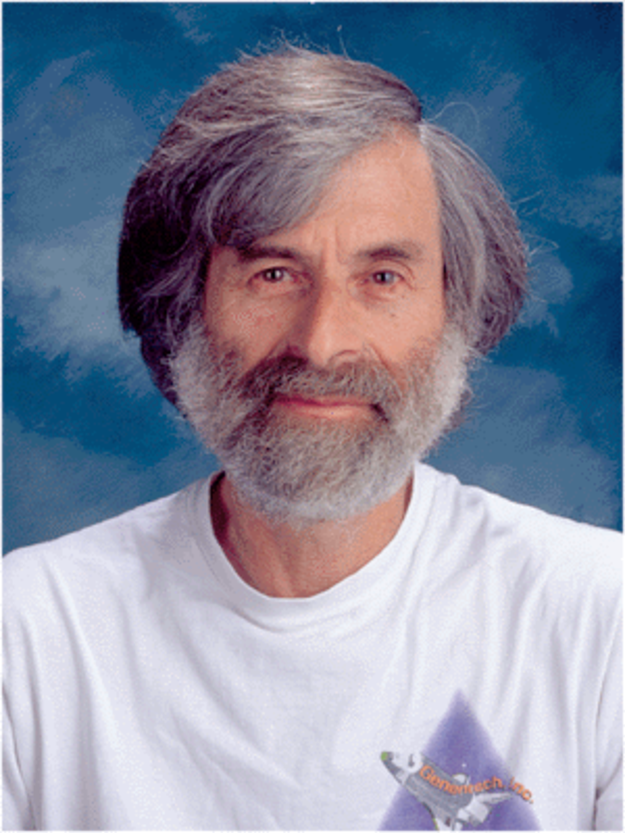
\includegraphics[width=\linewidth]{figs/leslie}
  \end{minipage}
  \hfill
  \begin{minipage}{.6\linewidth}
    \raggedright
    \begin{small}
      PhD 1972 (Brandeis University), Mathematics

      \begin{itemize}
      \item Mitre Corporation, 1962--65
      \item Marlboro College, 1965--69
      \item Massachusets Computer Associates, 1970--77
      \item SRI International, 1977--85
      \item Digital Equipment Corporation/Compaq, 1985--2001
      \item Microsoft Research, since 2001
      \end{itemize}
    \end{small}
  \end{minipage}

\bigskip

  Pioneer of distributed algorithms

  \begin{small}
  \begin{itemize}
  \item Natl. Academy of Engineering,
    PODC Influential Paper Award, ACM SIGOPS Hall of Fame, LICS Award,
    IEEE John v. Neumann medal, \ldots
  \item honorary doctorates (Rennes, Kiel, Lausanne, Lugano, Nancy)
  \end{itemize}
  \end{small}
\end{frame}

\begin{frame}
  \frametitle{\tlaplus{} specification language\hspace*{1.5cm}{\normalsize\url{http://tlaplus.net}}}

  \begin{minipage}{0.27\linewidth}
    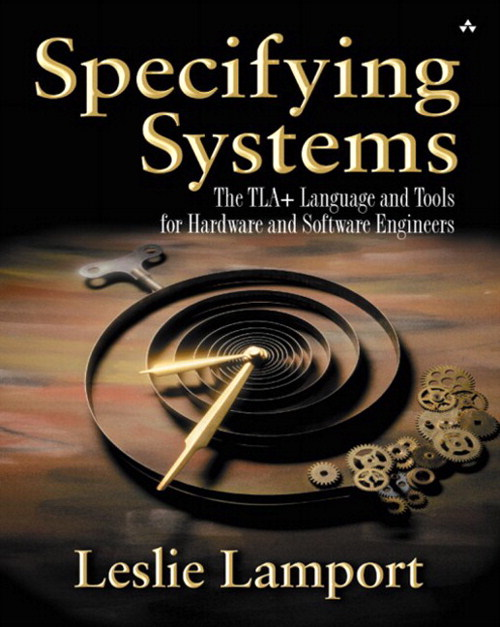
\includegraphics[width=\linewidth]{figs/tla-book-cover}
  \end{minipage}
  \hfill
  \begin{minipage}{.7\linewidth}
    \raggedright

    \begin{small}
    \begin{itemize}
    \item formal language for describing and reasoning about
      distributed and concurrent systems
\medskip
    \item based on mathematical logic and set theory\\
      plus linear time temporal logic TLA
\medskip
    \item book: Addison-Wesley, 2003\\
      (free download for personal use)
\medskip
    \item supported by tool set (\tlaplus{} toolbox)      
    \end{itemize}
    \end{small}
  \end{minipage}

  \pause
  \bigskip

  \tc{dkblue}{Some other publications}

  \begin{footnotesize}
  \begin{itemize}
  \item Y. Yu, P. Manolios, L. Lamport: \emph{Model checking \tlaplus{}
      Specifications}. CHARME 1999, pp. 54-66, LNCS 1703.
  \item S. Merz: \emph{The Specification Language \tlaplus}. In: Logics of
    Specification Languages (D. Bj{\slasho}rner, M. Henson, eds.), Springer
    2008, pp. 401-451.
  \item K. Chaudhuri, D. Doligez, L. Lamport, S. Merz: \emph{Verifying Safety
    Properties with the \tlaplus{} Proof System}. IJCAR 2010, pp. 142-148, LNCS 6173
  \end{itemize}
  \end{footnotesize}
\end{frame}
